\documentclass{article}

\usepackage{graphicx}

\title{The effect of pipeline-collection-diversity on performance}

\author{Data Machines Corporation}

\begin{document}

\maketitle

\abstract{Have performers who have submitted \emph{diverse}
  collections of pipelines tended to have performed better than those
  who have submitted less diverse collections of pipelines?  The answer
  is: \emph{yes, there has existed a measurable improvement in best
    score with diversity, but the effect-size is small enough that it
    may not be of any consequence.}}

\section{Results}
See Figure 1 below.
\begin{figure}
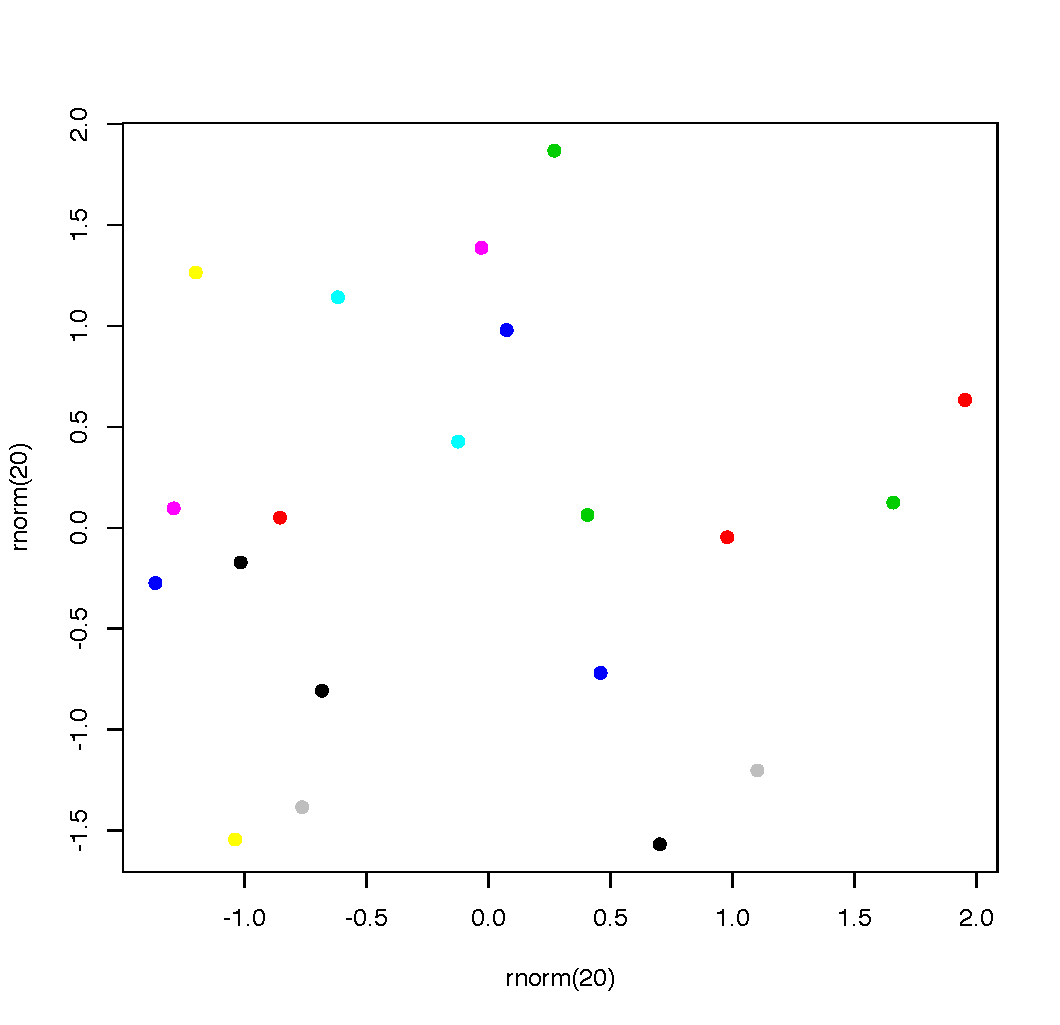
\includegraphics{heatmap.pdf}
\caption{This is the caption.}
\end{figure}

\section{Quantifying pipeline-collection-diversity}
  Before we define the \emph{diversity of a collection of pipelines},
  we must define the \emph{distance between a pair of pipelines}.
  Each possible primitive is given a letter in a large alphabet, and
  we define the distance between two pipelines as the Levenshtein edit
  distance between the pair: the minimum number of substitutions,
  insertions, and deletions, needed to make the two sequences
  identical.

  We considered several measures of collection diversity, looking at
  synthetic data to see if our measures made sense.  We achieved most
  success by concatenating the edit distances (between all pairs of
  pipelines in the collection) into a vector and defining the
  diversity as the \emph{norm} of this vector.  But this statement
  does not yet pin down the concept of diversity, because many notions
  of norm exist.

  Common norms are the $l_1$ norm, the $l_2$ norm and the $l_\infty$
  norm.  Indeed, the $l_p$ norm exists for any real number $p$ which
  is greater than or equal to 1.  All of these choices define a
  continuum of alternative notions of diversity.

  The $l_1$ norm defines diversity as the \emph{sum} of the edit
  distances.  Technically $l_1(v)$ is the sum of the absolute values
  of the components of $v$.  But in our case, all edit distances must
  remain positive, so it is not necessary to require absolute values.

  On the other extreme, $l_\infty$ defines diversity as the largest
  edit distance between all pairs of pipelines in the collection
  (i.e.\ the \emph{diameter of the collection}).  Notice that
  $l_\infty$ does indeed define diversity differently from $l_1$.  The
  two norms will rank two collections differently if one has many
  pairs of pipelines at small to moderate distance but no pairs at
  large distance, whereas the other has a few pairs at large distance,
  and the rest at zero distance.  (Distinct pipelines can have zero
  distance if they have the same sequence of primitives but possibly
  different values for hyperparameters.)  It should be evident that
  these two measures define alternative, but valid and useful notions
  of diversity.

  For increasing values of $p$ between 1 and $\infty$, the $l_p$
  measure of diversity combines both notions while placing increasing
  weight on the second notion when trading off the two definitions.
  Partway between $l_1$ and $l_\infty$ is the $l_2$ norm which is the
  Euclidean length of the vector of Levenshtein edit distances.

  What notion of diversity should be used?  If only one notion is
  reported, $l_2$ provides a nice compromise, but if two are reported,
  $l_1$ and $l_\infty$ together give the most information about the
  collection.

  \section{Significance}
  We claim that the effect of diversity on the Winter 2020 evaluation
  was measureable, meaning statistically significant.

  \section{Quantifying the small effect size}
  We claim that the effect size is small enough that it may be
  inconsequential.
  
  \end{document}


  
